
\documentclass[12pt,italian,a4paper,oneside,openright]{book}
\usepackage{url,amsfonts,epsfig}
\usepackage[italian]{babel}
\usepackage[latin1]{inputenc}
%\usepackage[format=hang,font=footnotesize]{caption}
\usepackage{vmargin}
\usepackage{amsmath}
\usepackage{indentfirst}
\usepackage{graphicx}
\usepackage{textcomp}
%\usepackage{algorithm,algorithmic}
\graphicspath{{img/}}
\usepackage[hyperindex]{hyperref} %per l'indice interattivo
\hypersetup{colorlinks=true, linkcolor=black} %per colorare i link
\DeclareGraphicsRule{.jpg}{jpg}{}{} %da commentare per il PDF

\begin{document}
\pagenumbering{Roman}

%%%% Opzione per interlinea 2
\baselineskip 1.5em

%% FRONTESPIZIO
{ \thispagestyle{empty}

\vskip 1cm \large \centerline{\textsc{Universit\`a degli Studi di
Napoli ``Parthenope''}}

\centerline {\textsc{Dipartimento di Scienze e Tecnologie}}

\centerline {\small\textsc{Corso di laurea Triennale in Informatica}}

\begin{center}

\includegraphics[scale=0.5]{logo_parthenope.png}
\end{center}

\vskip 0.5cm

\large \centerline {\textsc{Programmazione 3 e Laboratorio di Programmazione 3}}

\vskip 0.5cm

\Large \centerline {Distributore bevande}


\vskip 4.5cm


\large
\begin{minipage}[t]{7cm}
\textsc{Docente}

Prof. Angelo Ciaramella

\end{minipage}
\hfill
\begin{minipage}[t]{6cm}
\hfill \textsc{Candidato}

\hfill Vittorio Fones 0124/1384
\end{minipage}

\vskip 2.0 cm \Large \centerline {Anno Accademico 2018-2019}
\vfill \eject}

% fine frontespizio

\markboth{Indice}{Indice}
\tableofcontents
\listoffigures
\newpage

\pagenumbering{arabic}
\thispagestyle{headings}
\chapter{Introduzione} \label{cap0}
Il progetto in esame \textbf{\`e un simulatore di un distributore automatico di bevande}, abbreviato
D.V.M.\footnote{Drink Vending Machine. In inglese vending machine \`e il distributore automatico}.
L'applicativo prevede due utilizzi, uno da \textbf{utilizzatore} e il secondo come \textbf{super utente}.
Per praticit\'a l'utente non ha bisogno di effettuare un accesso tramite username e password, sebbene sia identificabile
come vedremo. Si definisco di seguito gli attori e i loro task come da traccia.\newline
\textbf{L'utente} pu\`o:
\begin{itemize}
    \item scegliere, prelevare e pagare una bevanda. Il pagamento pu\`o avvenire
    secondo le modalit\`a: contanti (5,10,20,50 centesimi, 1 e 2 euro), chiavetta
    ricaricabile o carta di credito;
    \item ricaricare una chiavetta inserendo contanti (5,10,20,50 euro).
\end{itemize}

\textbf{L'amministratore} pu\`o:
\begin{itemize}
    \item periodicamente aggiungere bevande alla scorta. Il sistema controlla automaticamente se la bevanda
    \`e sotto scorta (minore di 1 litro);
    \item  definire il prezzo per ogni tipo di bevanda;
    \item  fare un report sui consumi mensili delle diverse tipologie di bevande;
    \item aggiungere una nuova tipologia di bevanda partendo da quelle gi\`a esistenti (e.g., th\`e con limone);
\end{itemize}
\def\baselinestretch{1}
\chapter{Scelte progettuali} \label{cap1}
\def\baselinestretch{1.66}
\section{Tecnologie usate}
Il progetto \`e stato sviluppato come una web application, utilizzando le note tecnologie Servlet e JSP
eseguite nel web server Apache Tomcat. Per le JSP\footnote{JavaServer Pages},
ovvero le pagine dinamiche in formato HTML, sono state sviluppate usando la recente notazione con tag JSTL che rende 
la lettura e interpretazione (da parte del programmatore) pi\`u semplice. 
I dati sono memorizzati in un database relazionale, usando PostgreSQL come RDBMS. L'interfaccia con la
quale si comunica alla base di dati \`e offerta dal noto framework Open Source
Hibernate, per tanto il cambiamento della sorgente dati \`e immediato,
baster\`a modificare il file di configurazione .xml\footnote{Scelta arbitraria tra la configurazione del
file .xml o la codifica nella classe atta alla configurazione}.
\newpage
\section{Architettura e logica di funzionamento}
Lo sviluppo delle web application \`e per lo pi\`u basato seguendo un pattern noto come MVC (Model - view - controller). Il compito di questo pattern \`e di dividere la presentazione,
ovvero l'interfaccia utente, e la sua logica di come manipola i dati e li presenta all'utilizzatore dell'applicativo.
\begin{figure}[ht]
    \centering
    \includegraphics[scale=0.4]{img/MVC-Process.eps}
    \caption{Diagramma di interazione del pattern MVC.}
\end{figure}

Il componente \textbf{controller} \`e dato dalle classi che estendono le Servlet: prendono i dati forniti dall'utente
e contribuiscono al normale flusso dell'applicazione, interagendo con i dati.
Il \textbf{model}, \`e composto dai \textbf{data model}, identificati pi\`u semplicemente come \textbf{Java Bean} (classi con attributi privati e metodi Getter e Setter) e dalle \textbf{actions} (modificatori dei data model).
Nel caso di questo progetto le actions e i controller sono le servlet che scambiandosi i parametri delle chiamate Http usando i metodi Get e Post, aggiornano le \textbf{views}: i file JSP che utilizzando EL\footnote{Expression Language}.

\chapter{Conclusioni} \label{cap3}
\def\baselinestretch{1.66}
\section{Database}
Il database mostrato di seguito \`e usato per conservare le informazioni di accesso degli
amministratori, i prodotti da vendere, gli acquisti delle bibite e le chiavi ricaricabili.
Quest'ultime sono le uniche che contengono informazioni sugli utenti, poich\`e a seguito di assunzioni
si \`e pensato che gli utenti vengano registrati dal DBA, cos\`i come gli amministratori. A
seguito di ci\`o nello sviluppo non \`e stato preso in considerazione una pagina per la registrazione e un metodo nella classe Dao per l'eliminazioni di tuple.

\begin{figure}[ht]
    \centering
    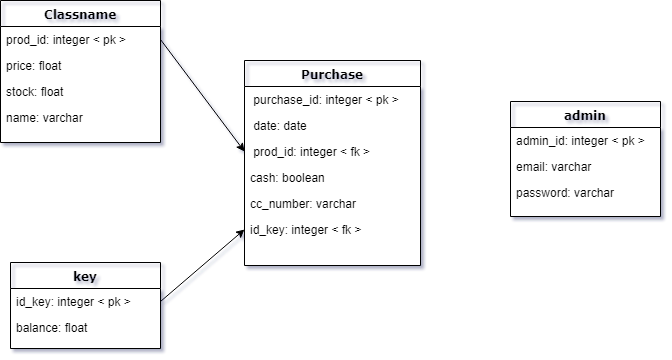
\includegraphics[scale=0.5]{img/database.png}
    \caption{Database relazionale.}
\end{figure}

\chapter{Diagramma delle classi} \label{cap2}
\def\baselinestretch{1.66}
Di seguito vengono illustrati i \textbf{diagrammi delle classi} che fanno uso di specifici pattern. Per quanto riguarda le servlet, poich\'e queste hanno tutte le stesse \textbf{signature} si \`e deciso di mostrare solamente
quelle che mostrano le informazioni alle views, piuttosto che elencare tutti i controller delle
\textbf{rotte}\footnote{In ambito web le rotte non sono altro che le risorse della url}.
\section{Servlet come controller}
\begin{figure}[ht]
    \centering
    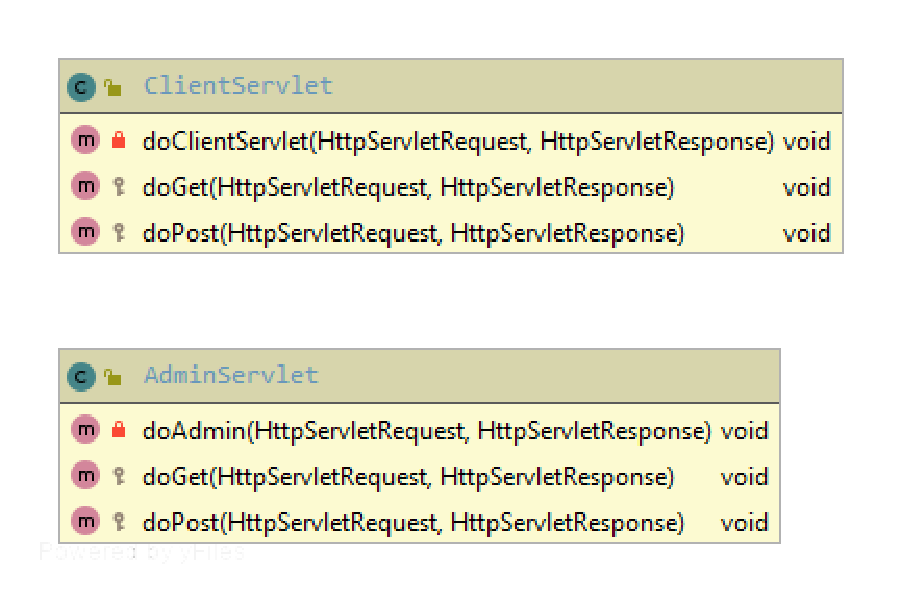
\includegraphics[scale=0.6]{img/servlet.eps}
    \caption{Servlet principali per le informazioni da passare alle views.}
\end{figure}
\newpage
\section{Template Method e Singleton}
Metodi per le operazioni del database creati con il template method e singleton. L'unica
classe usata per interrogare il database sar\`a \textbf{GenericDao} che \`e una classe templata.
\begin{figure}[ht]
    \centering
    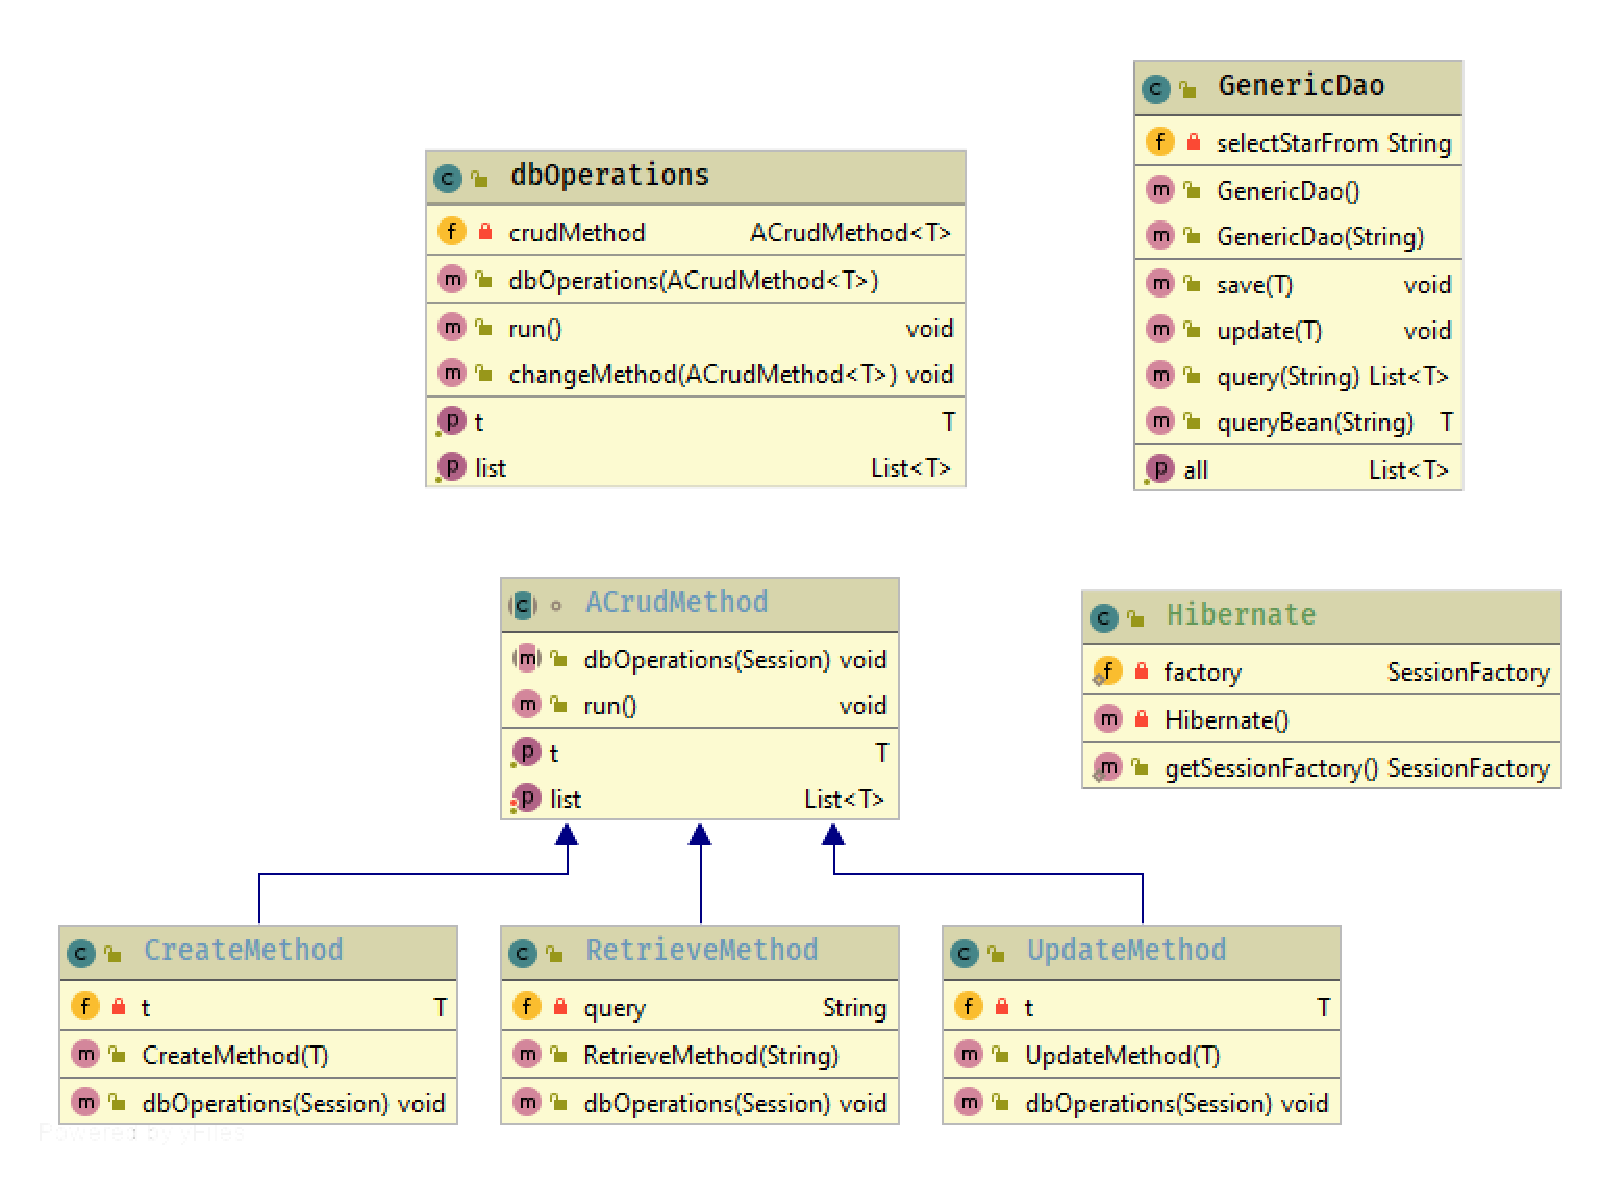
\includegraphics[scale=0.6]{img/tm.eps}
    \caption{Diagramma dei metodi templati.}
\end{figure}
\newpage
\section{Java Bean}
Principali Java Bean usate per "mappare" le entit\`a del database
\begin{figure}[ht]
    \centering
    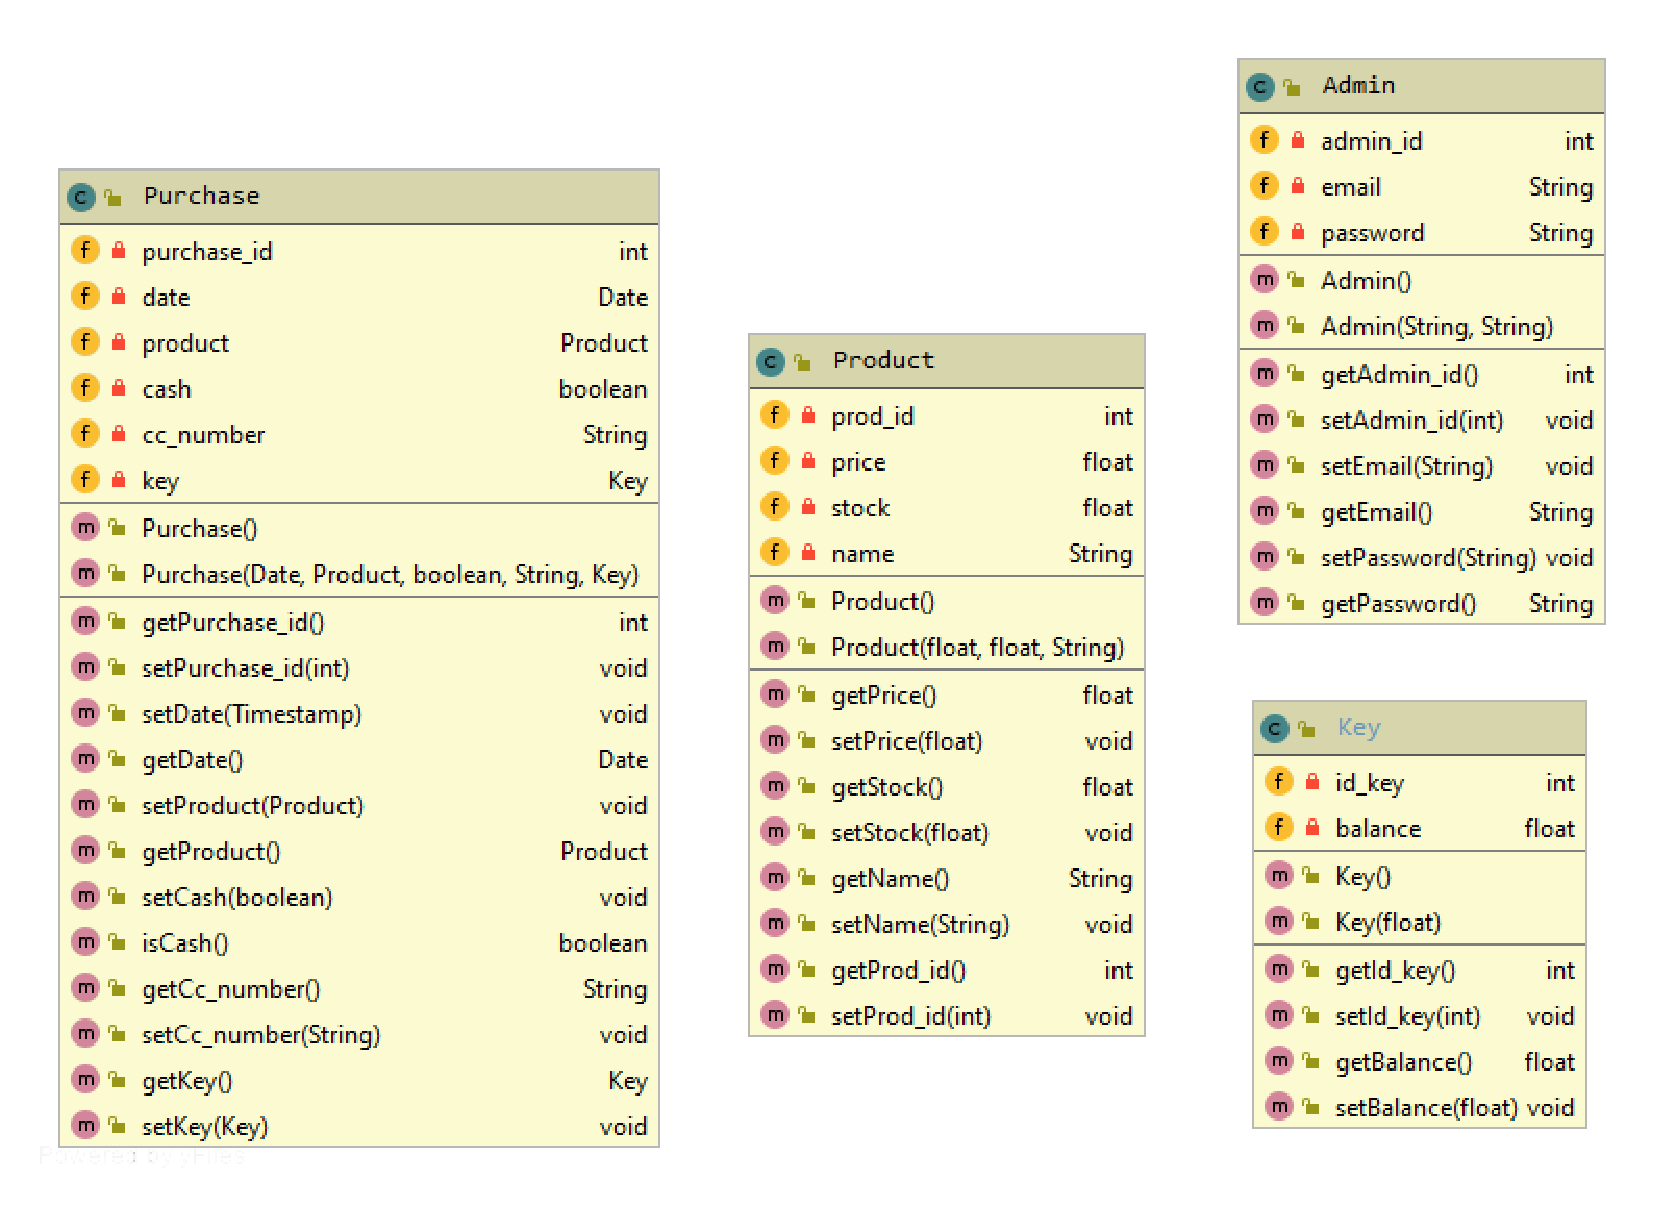
\includegraphics[scale=0.5]{img/javabean.eps}
    \caption{Java bean.}
\end{figure}
\newpage
\section{Chain of Responsibility}
Controllo dei metodi di pagamento tramite catena di responsabilit\`a.
\begin{figure}[ht]
    \centering
    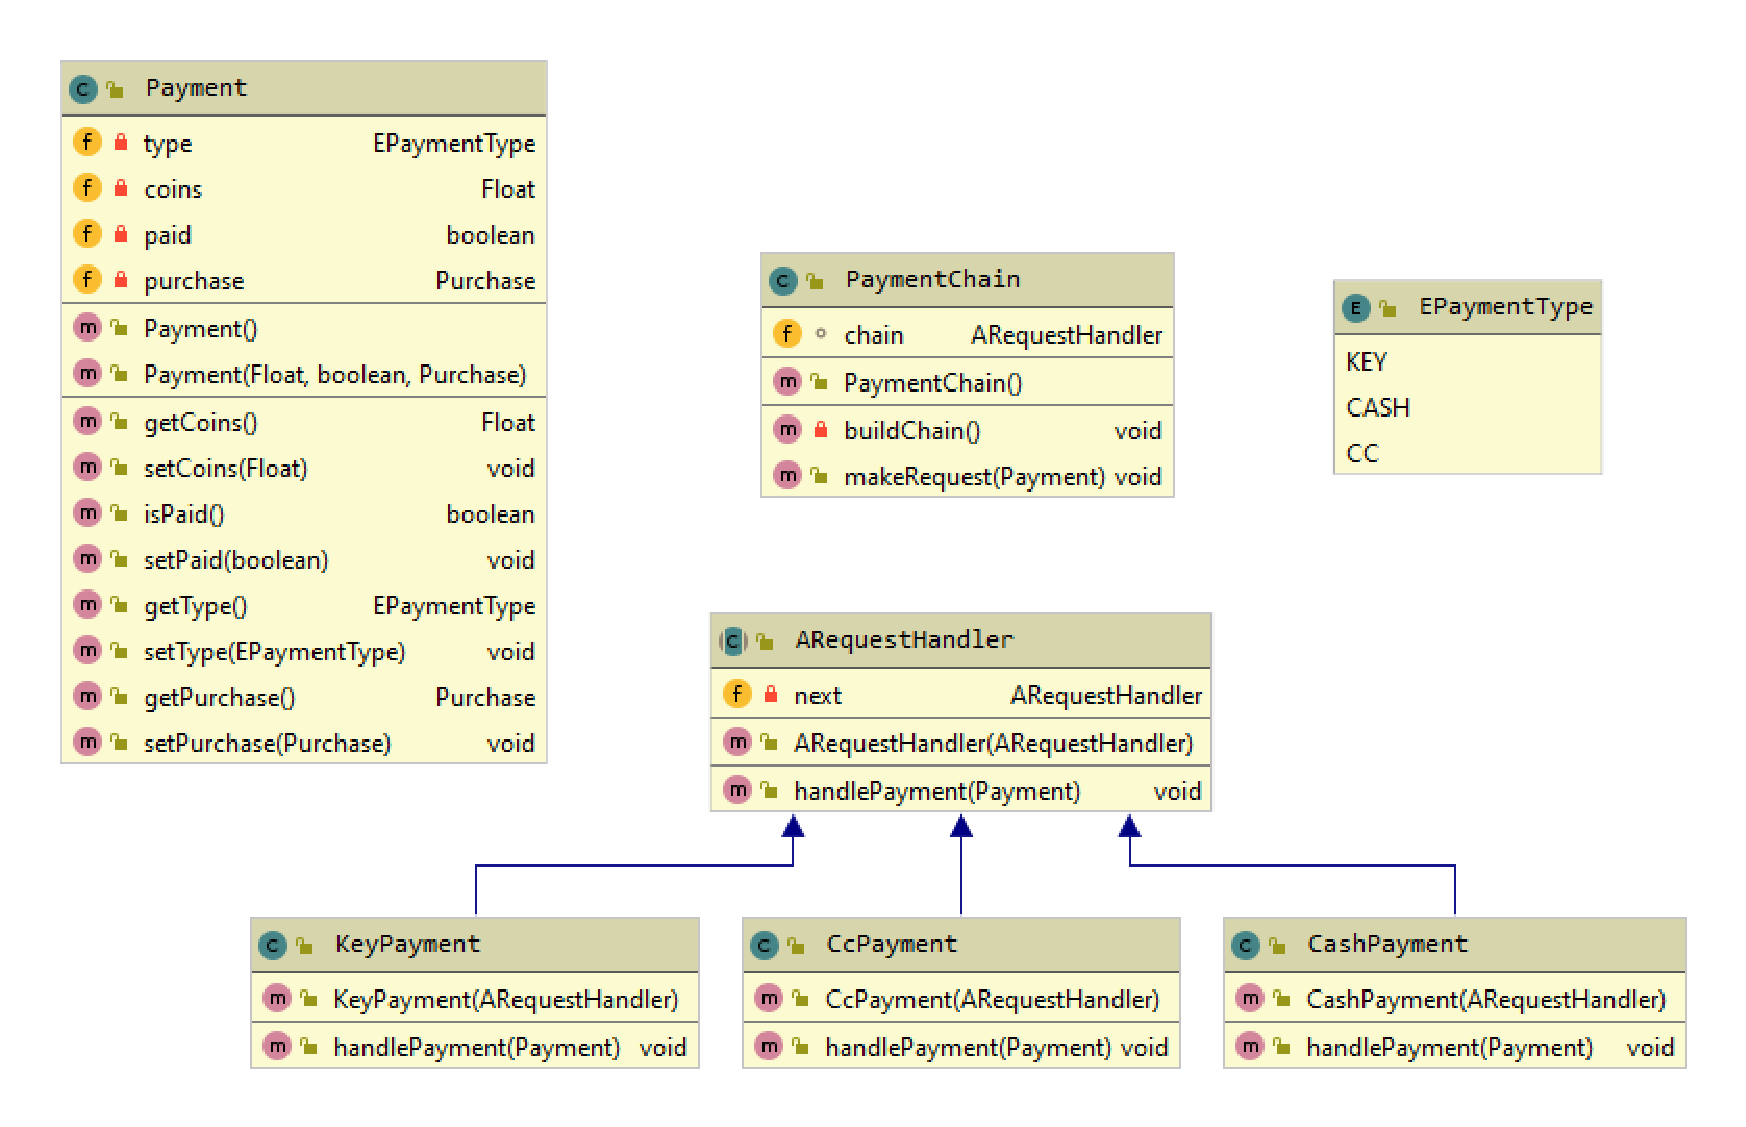
\includegraphics[scale=0.5]{img/cor.eps}
    \caption{Diagramma della Chain of Responsibility.}
\end{figure}
\newpage

\begin{thebibliography}{30}
    \bibitem{TOMCAT} Apache Tomcat \\
        \url{https://tomcat.apache.org/}
    \bibitem{H8} Hibernate middleware\\
        \url{https://hibernate.org/}
    \bibitem{WIKI} Wikipedia\\
        \url{https://wikipedia.org}
    \bibitem{BIGG} Google\\
        \url{https://www.google.com}
    \bibitem{SO} Stackoverflow\\
        \url{https://stackoverflow.com}
\end{thebibliography}

\newpage
\pagestyle{plain}


\end{document}
